% !TeX Options = -shell-escape

\documentclass[10pt]{beamer}

\usetheme[progressbar=frametitle, block=fill]{metropolis}
\usepackage{xcolor}
\usepackage{multirow}
\usepackage{pgfpages}
\usepackage{pifont}
\usepackage[utf8]{inputenc}
\usepackage[T1]{fontenc}
\usepackage{csquotes}
\usepackage[english]{babel}
\newcommand{\cmark}{\ding{51}}
\newcommand{\xmark}{\ding{55}}
\setbeamertemplate{note page}{\insertnote}
%\setbeameroption{show notes on second screen=left}

\setbeameroption{hide notes}
\definecolor{amethyst}{rgb}{0.5, 0.4, 1.0}
\definecolor{amethystgrey}{rgb}{0.85, 0.85, 1.0}
\definecolor{amethystdark}{rgb}{0.4, 0.3, 0.9}
\definecolor{orangedark}{rgb}{0.0, 0.9, 0}
\definecolor{titlebg}{HTML}{fbf8ff}
\definecolor{font}{HTML}{23373b}
\setbeamercolor{frametitle}{fg= font, bg=titlebg}
\setbeamercolor{progress bar}{ fg = amethyst, bg= amethystgrey }
\setbeamercolor{alerted text}{fg=amethystdark}

\usepackage{booktabs}
\usepackage[scale=2]{ccicons}

\usepackage{minted}

\usepackage{pgfplots}

\usepackage{xspace}

\title{Coroutines in the C++}
\subtitle{Introduction to the C++ coroutines}
\date{}
\author{Dawid Pilarski}
\institute{dawid.pilarski@panicsoftware.com \\ \href{http://blog.panicsoftware.com}{blog.panicsoftware.com} \\ dawid.pilarski@tomtom.com}

\begin{document}

\maketitle

\section{Introduction}
\begin{frame}{Agenda}
	\tableofcontents
\end{frame}

\begin{frame}{Questions...}

\vfill
\centerline{Ask questions any time.}
\centerline{Don't be afraid to interrupt me :)}
\vfill

\end{frame}

\begin{frame}{Who am I?}
			\centering \alert{Dawid Pilarski}
			\vskip 1em
	\begin{columns}[onlytextwidth]
		\begin{column}{0.7\textwidth}
			\begin{itemize}
				\item Senior Software Developer in TomTom
				\item Member of the ISO/JTC1/SC22/WG21
				\item Member of the PKN KT {\tiny(programming languages)}
				\item C++ blog writer
			\end{itemize}
		\end{column}
		\begin{column}{0.29\textwidth}
				
\includegraphics[width=\linewidth]{Dawid_Pilarski.jpg}				
		\end{column}	
	\end{columns}
\end{frame}

\section{Why do we need coroutines?}

\begin{frame}{What are the coroutines?}
\vfill

\begin{description}
	\item [Subroutine] Is a sequence of program instructions that performs a specific task, packaged as a unit.
	\item [Function] Is a subroutine
	\item [Coroutine] Is generalization of the function.
\end{description}

\vfill
\end{frame}

\begin{frame}{What are the coroutines?}
	\alert{\only{Function}<1>\only{Coroutine}<2->} can be:
	\begin{itemize}
		\item called
		\item returned from
		\item<2-|alert@2> \alert<+>{suspended}
		\item<3-|alert@3> resumed from
		\item<4-|alert@4> created
		\item<5-|alert@5> destroyed
	\end{itemize}
\end{frame}

\begin{frame}{Coroutine flowchart}

\begin{columns}
\begin{column}{0.48\linewidth}
  \centering
  Function's flow:
  \vskip 2em
  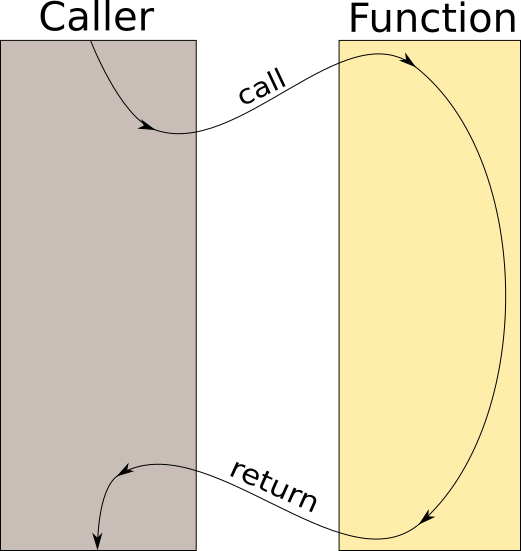
\includegraphics[width=0.8\linewidth]{graphics/function-call.png}
\end{column}
\begin{column}{0.48\linewidth}
  \centering
  Coroutine flow:
  \vskip 2em
  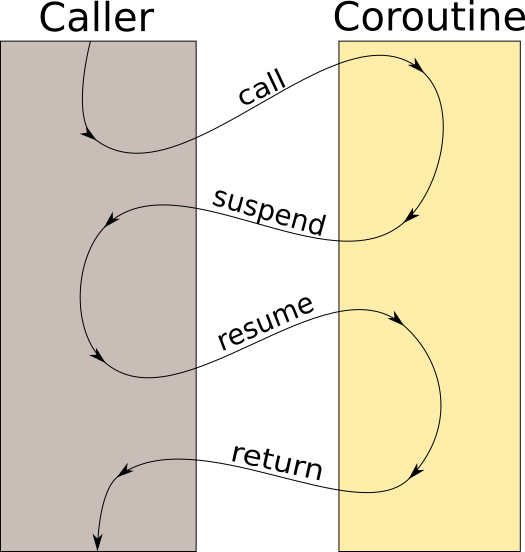
\includegraphics[width=0.8\linewidth]{graphics/coroutine-workflow.png}
\end{column}

\end{columns}

\end{frame}

\begin{frame}{Coroutines use cases}
	\begin{itemize}
		\item cooperative multitasking
		\item generators
		\item easier state-based computations
		\item prevent active waiting in the programs
	\end{itemize}
\end{frame}

\section{Why do we need language support for the coroutines?}
\begin{frame}{C++ coroutines vs library coroutines}
\begin{columns}[t]
\begin{column}{0.48\linewidth}
  \centering Language based
  \vskip 2em
  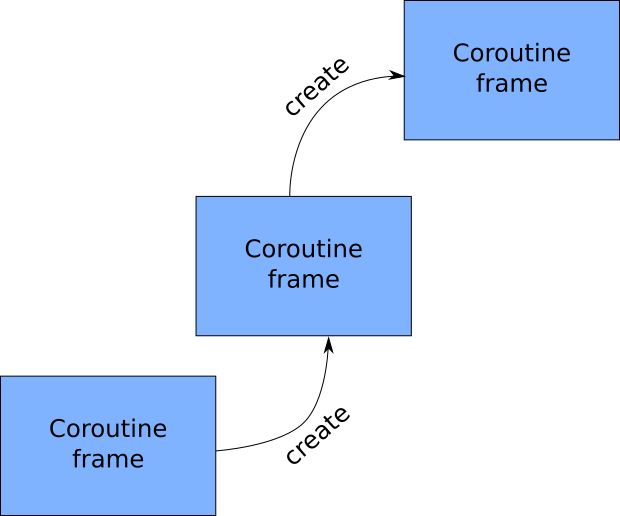
\includegraphics[width=.8\linewidth]{graphics/cppcoro-creation.png}
\end{column}

\begin{column}{0.48\linewidth}
\centering
  Library based
  \vskip 2em
  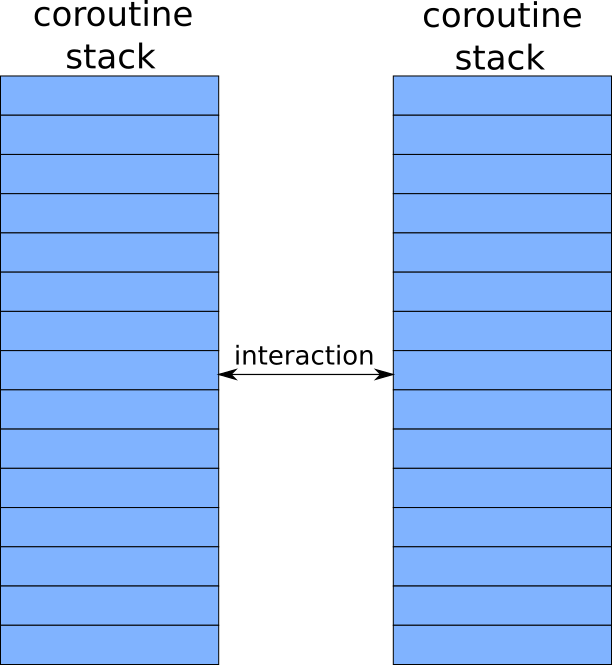
\includegraphics[width=.8\linewidth]{graphics/coroutine-interaction.png}
\end{column}
\end{columns}

\end{frame}

\begin{frame}{C++ vs library - summary}
  \begin{itemize}[<+- |alert@+>]
  \item Need to allocate the stack for the Fiber/Coroutine
  \item Can be suspended from the top level functions and below
  \item Allocation of the memory in advance
  \item One allocation per whole stack.
  \end{itemize}
\end{frame}

\begin{frame}{C++ vs library - summary}
\begin{columns}[t]
  \begin{column}{0.48\linewidth}

  \centerline{\alert{Boost.Fiber}}
  \vfill
  \begin{itemize}
  \item Need to allocate \alert{the stack} for the Fiber/Coroutine
  \item Can be suspended from the \only{top level functions and below}<1>\only{\alert{top level functions and below}}<2->
  \item Allocation of the memory \only{in advance}<1-2>\only{\alert{in advance}}<3->
  \item \only{One}<1-3>\only{\alert{One}}<4-> allocation per whole stack.
  \end{itemize}
  \end{column}
  \begin{column}{0.48\linewidth}

  \centerline{\alert{built-in coroutines}}
  \vfill
  \begin{itemize}[<+->]
  \item Need to allocate \alert{the frame} for the Coroutine
  \item Can be suspended only from the \alert{top level function}
  \item \alert{Minimal} memory allocations 
  \item \alert{Multiple} allocations
  \end{itemize}
  \end{column}
  
  \end{columns}
\end{frame}

\section{How to implement your own coroutine types?}

\begin{frame}{What's the issue?}
	Creating custom coroutine type is not easy:
	\begin{itemize}[<+->]
		\item C++ provides keywords \alert{only}.
		\item \alert{Developer must implement} what keywords do.
	\end{itemize}

	\vfill

	\only{This means:}<3->
	\begin{itemize}[<+->]
		\item Implementation of promise\_type ({\fontfamily{ptm}\selectfont\texttildelow}6 functions)
		\item Implementation of the co\_await  keyword ({\fontfamily{ptm}\selectfont\texttildelow}3 functions)
	\end{itemize}

	\vfill

	\only{You need to remember to implement on average \alert{9 functions}.}<5>
\end{frame}

\begin{frame}{Coroutine declaration}
  \vfill
  \begin{center}
  \begin{minipage}{0.8\linewidth}
  \inputminted{c++}{code-examples/intro/declaration.hpp}
  \end{minipage}
  \end{center}
  \vfill

  \pause

  \begin{itemize}[<+->]
  	\item Whether the function is a coroutine depends on \alert{it's definition}.
  	\item If function is a coroutine it's \alert{return type must support coroutines}.
  \end{itemize}
  
\end{frame}

\begin{frame}{Promise\_type}
	Type supports coroutines \alert{if it has promise\_type}.
	\vfill

	promise\_type can be:
	\begin{itemize}
		\item member of the class
		\item member of the specialization of the coroutine\_traits<returned\_type>
	\end{itemize}
\end{frame}

\begin{frame}{Promise\_type}
	\centerline{Promise\_type controls coroutine's behavior.}
	\vfill

	\begin{columns}
		\begin{column}{0.48\linewidth}
			\begin{footnotesize}
			\begin{itemize}[<+-|alert@+>]
				\item \texttt{awaitable initial\_suspend();}
				\item \texttt{awaitable final\_suspend();}
				\item \texttt{return\_type get\_return\_object();}
				\item \texttt{void unhandled\_exception();}
			\end{itemize}
			\end{footnotesize}	
		\end{column}
		\begin{column}{0.48\linewidth}
			\begin{footnotesize}
			\begin{itemize}
				\item<1- |alert@1> \texttt{suspension at the beginning}
				\item<2- |alert@2> \texttt{suspension at the end}
				\item<3- |alert@3> \texttt{how to create \\ return\_type}
				\item<4- |alert@4> \texttt{handling unhandled exception}
			\end{itemize}
			\end{footnotesize}	
		\end{column}
	\end{columns}
\end{frame}

\begin{frame}{Keywords and promise\_type}
	Promise\_type is also responsible for keyword's actions:
	\vfill

	\begin{columns}
		\begin{column}{0.48\linewidth}
			\begin{footnotesize}
			\begin{itemize}[<+-|alert@+>]
				\item \texttt{co\_return V;}
				\item \texttt{co\_return;}
				\item \texttt{co\_yield V;}
			\end{itemize}
			\end{footnotesize}	
		\end{column}
		\begin{column}{0.48\linewidth}
			\begin{footnotesize}
			\begin{itemize}[<+-|alert@+>]
				\item<1- |alert@1> \texttt{void return\_value(V);}
				\item<2- |alert@2> \texttt{void return\_void();}
				\item<3- |alert@3> \texttt{awaitable yield\_value();}
			\end{itemize}
			\end{footnotesize}	
		\end{column}
	\end{columns}
\end{frame}

\begin{frame}{Implementing generator: the API}
	\inputminted[firstline=7, lastline=18, fontsize=\footnotesize]{c++}{code-examples/cppcoro/generator.cpp}
\end{frame}

\begin{frame}{Implementing generator: the promise\_type}
	\inputminted[firstline=20, lastline=41, fontsize=\scriptsize]{c++}{code-examples/cppcoro/generator.cpp}
\end{frame}

\begin{frame}{Implementing generator}
	\inputminted[fontsize=\scriptsize]{c++}{code-examples/cppcoro/generator_impl.cpp}
\end{frame}

\begin{frame}{co\_await}
	In order to support co\_await expressions, the argument (awaitable) must:
	\begin{itemize}
		\item have \texttt{awaiter operator co\_await} defined, or
		\item have global \texttt{awaiter operator co\_await(T)} support, or
		\item implement 3 functions:
		\begin{itemize}
			\item \texttt{bool await\_ready()}
			\item \texttt{await\_suspend(coroutine\_handle<T>)} returning
			\begin{itemize}
				\item void 
				\item bool
				\item another \texttt{coroutine\_handle}
			\end{itemize}
			\item \texttt{T await\_resume()}
		\end{itemize}
	\end{itemize}
\end{frame}

\begin{frame}{co\_await example - single\_consumer\_event}
	\inputminted[lastline=20, fontsize=\scriptsize]{c++}{code-examples/cppcoro/single_consumer_event.hpp}
\end{frame}

\begin{frame}{co\_await example - single\_consumer\_event}
	\inputminted[firstline=22, fontsize=\scriptsize]{c++}{code-examples/cppcoro/single_consumer_event.hpp}
\end{frame}

\section*{Thank you for attention}

\begin{frame}{Bibliography and further reading}
\begin{columns}
\begin{column}{0.48\linewidth}
	\begin{itemize}
		\item Lewiss Baker's Assymetric transfer blog
		\item newest C++ draft
		\item My blog - blog.panicsoftware.com
	\end{itemize}
\end{column}
\begin{column}{0.48\linewidth}
	\begin{itemize}
		\item James McNellis - "Introduction to the C++ Coroutines"
		\item Gor Nishanov - any video about the coroutines
		\item Toby Allsopp - "Coroutines: what can't they do?"
	\end{itemize}
\end{column}

\end{columns}
\end{frame}

\begin{frame}{Questions?}
\vfill
\centering Questions?
\vfill
\end{frame}

\end{document}